%!TEX root = ../Studienarbeit.tex

\chapter{Einleitung}

Multikopter bezeihungsweise Quadrokopter haben in den letzten Jahren sowohl im privaten als auch im kommerziellen einen konstanten Wachstum erlebt. So sind beispielsweise in den vereinigten Staaten von Amerika zum Stand vom 31. Mai 2022 über 865.000 Multikopter regestriert. Dabei sind über 500.000 Multikopter für die private und über 300.000 für die kommerzielle Nutzung registriert. \cites{droneregistrationFAA}{dronestat1}{dronestat2}{dronestat3}

Quadrokopter lassen dabei in zwei Arten einteilen. Zum einen die Consumerquadrokopter welche viele  Sensoren und dazugehörige Unterstützungfunktionen haben, damit diese leicht durch ungeübte Personen geflogen werden können. Ein beispiel für einen Quadrokopter dieser Art währe die Mavic 3 Classic von dem Unternehmen DJI. Diese hat beispielsweise Sichtsensoren welche nach unten, oben, vorne und hinten ausgerichtet sind, um Objekte im Flugfeld auszuweichen. Ebenso unterstützt dieser Quadrokopter ebenso den automatischen Rückflug an den Startpunkt. Auch ist ein System implementiert, wodurch der Quadrokopter beim loslassen der Steuerknüppel an der Fernsteuerung, an dem aktuellen Ort mit der aktuellen Höhe verhart bis der Quadrokopterpilot wieder eingreift. \cite{djiMavicClassic}

Die zweite Art von Quadrokoptern sind sogenannte Freestyle- beziehungsweise Rennquadrokoptern. Diese sind im Gegensatz zu den Consumerquadrokopter dazu ausgelegt möglichst leicht zu sein und so wenig Unterstützungfunktionen zu haben wie möglich, um schnelle und beindruckende Manöver machen zu können. Dafür haben diese Quadrokopter drei mögliche Flugmodi. Zum einen den Flugmodus \textit{Angle Mode} dabei wird der Quadrokopter ab einen Neigungswinkel automatisch begränzt wodurch Loopings und Rollen des Quadrokopters unterbunden werden und bei Zentrierung der Steuerknüppel der Quadrokopter wieder in die Ausgangslage zurückdreht. Der zweite Flugmodus ist der \textit{Horizon Mode}, dieser bietet wie der \textit{Angle Mode} die Funktion, dass sich der Quadrokopter wieder zur Ausgangslage zurückdreht wenn die Steuerknüppel in die zentrale Stellung zurückgebracht werden. Jedoch können in diesen Flugmodus Loopings und Rollen gemacht werden. Der letzte verfügbar Flugmodus ist der \textit{Air beziehungsweise Acro Mode}. In diesen Modus muss der Pilot sich um das Ausrichten der Drohne in alle Drehrichtungen kümmern, da bei loslassen der Steuerknüppel die vorhanden Winkel des Quadrokopters beibehalten werden. Dieser Modus wird von Freestyle und Rennpiloten verwendet. In Abbildung \ref{fig:flugmodi} ist eine Übersicht aller Flugmodi zu sehen. \cite{wedioFlugmodi}

\begin{figure}[h]
    \centering
    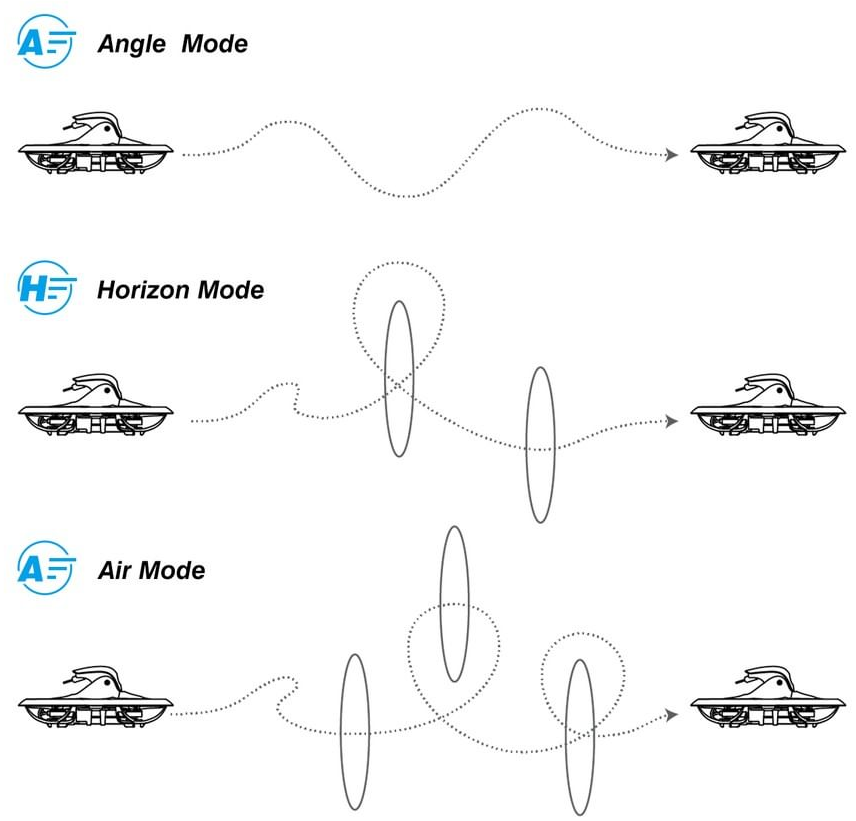
\includegraphics[width=.25\paperheight]{flugmodi}
    \caption{\acs{HID} Verfügbaren Flugmodi bei Freestyle beziehungsweise Rennquadrokoptern; angepasst von \cite{betafpvFlugmodi}}
    \label{fig:flugmodi}
\end{figure}

Neben dem Multikopterfliegen stellt für Renn- und Freestyle-Quadrokopterpiltoen das Training ein wichtiger Bestandteil dar, um das Handling des Quadrokopters im \textit{Air beziehungsweise Acro Mode} zu verbessern. Das Training kann in zwei Varianten durchgeführt werden. Der Quadrokopterpilot trainiert entwerder am Flugplatz. Hier können aber durch Abstürze hohe Reperaturkosten und lange Reperaturzeiten entstehen. Oder der Quadrokopterpilot trainiert im Simulator am Rechner, wo diese Arbeit ansetzen soll.

\section{Motivation}

Da in den letzten Jahren das Unternehmen Apple Tablets mit leistungsstarken Prozessoren, welche ursprünglich für Notebooks und Desktops gedacht waren, entwickelt hat \cite{appleM2IPad}, wäre es wünschenswert Simulatoren für die immer leistungsfähigeren mobilen Geräte bereitzustellen. Für das Training am Simulatoren sollte jedoch die gewohnte Fernsteuerung der Quadrokoptern verwendet werden. Die Verwendung der gewohnten Fernsteuerung an Computern bieten einige Hersteller an, indem sich die Fernsteurung per USB als USB-\acs{HID}-Joystick identifiziert \cite{opentxJoystick}. Das Problem hierbei ist jedoch, dass die Verbindung mittels USB mit mobilen Geräten nur eingeschränkt beziehungsweise umöglich ist. Beseitigt werden kann dieses Problem bei einigen Fernsteuerung mit Modulschächten \cite{opentxModulbay}, mit Hilfe derer die Tasten- und Joysticksignale über andere Funkstandard übertragen werden können.

Ziel der Arbeit ist es daher eine Hardware-Erweiterungsmodul für Multikopterfernsteuerungen zu entwickeln, womit sich über ein andere Übertragungsart als USB die Fernsteuerung mit Geräten für das Training im Simulator verbunden werden kann.

\section{Stand der Technik}

Damit Fernsteuerungen von Quadrokoptern an Computern für das Training am Simulator verwendet werden können, gibt es zurzeit drei Möglichkeiten. Die erste Möglichkeit ist es die Fernsteuerung von einigen Herstellern mittels USB zu verbinden. Dadurch wird die Fernsteuerung am Computer als USB-\acs{HID}-Joystick erkannt\cite{opentxJoystick}. Die zweite Möglichkeit ist es, den Quadrokopter auf dem die Firmware Betaflight vorhanden ist mittels USB anzustecken und diesen als Empfänger für die Fernsteuerung zu verwenden \cite{betaflightHID}. Da diese zwei Möglichkeiten jeweils USB zur Datenübertragung verwenden sind diese Varianten nicht für alle Endgeräte geeignet. Die letzte Möglichkeit ist es an Fernsteuerung mit Erweiterungsmodulschacht ein Hardwaremodul zu verwenden, welches die Daten mittels Bluetooth überträgt. Hierbei ist als einziges bekanntes Modul von dem Unternhemen Orqa zu nennen \cite{orqaBluetoothModule}. Dieses Modul ist jedoch nur für Modulschächte des Typs JR geeignet und nicht für Modulschächte des Typs Lite.